% \documentclass[a4paper,dvipsnames]{article}

% \addtolength{\hoffset}{-2.25cm}
% \addtolength{\textwidth}{4.5cm}
% \addtolength{\voffset}{-3.25cm}
% \addtolength{\textheight}{5cm}
% \setlength{\parskip}{0pt}
% \setlength{\parindent}{0in}

% %----------------------------------------------------------------------------------------
%	PACKAGES AND OTHER DOCUMENT CONFIGURATIONS
%----------------------------------------------------------------------------------------

%----------------------------------------------------------------------------------------
%		Generals
%----------------------------------------------------------------------------------------
\usepackage{fourier}
\usepackage{frcursive}
\usepackage[T1]{fontenc} %Accents handling
\usepackage[utf8]{inputenc} % Use UTF-8 encoding
%\usepackage{microtype} % Slightly tweak font spacing for aesthetics
\usepackage[english, francais]{babel} % Language hyphenation and typographical rules

%----------------------------------------------------------------------------------------
%		Graphics
%----------------------------------------------------------------------------------------
\usepackage{xcolor}
\usepackage{graphicx, multicol} % Enhanced support for graphics
\graphicspath{{FIG/}}
\usepackage{wrapfig}

%----------------------------------------------------------------------------------------
%		Other packages
%----------------------------------------------------------------------------------------
\usepackage{hyperref}
\hypersetup{
	colorlinks=true, %colorise les liens
	breaklinks=true, %permet le retour à la ligne dans les liens trop longs
	urlcolor= bleu3,  %couleur des hyperliens
	linkcolor= bleu3, %couleur des liens internes
	plainpages=false  %pour palier à "Bookmark problems can occur when you have duplicate page numbers, for example, if you have a page i and a page 1."
}
\usepackage{tabularx}
\newcolumntype{M}[1]{>{\arraybackslash}m{#1}} %Defines a scalable column type in tabular
\usepackage{booktabs} % Enhances quality of tables
\usepackage{diagbox} % barre en diagonale dans un tableau
\usepackage{multicol}
\usepackage[explicit]{titlesec}


%----------------------------------------------------------------------------------------
%		Headers and footers
%----------------------------------------------------------------------------------------
\usepackage{fancyhdr} % Headers and footers
\pagestyle{fancy} % All pages have headers and footers
\fancyhead{}\renewcommand{\headrulewidth}{0pt} % Blank out the default header
\renewcommand{\footrulewidth}{0pt}
\fancyfoot[L]{} % Custom footer text
\fancyfoot[C]{\href{https://sacado.xyz/}{sacado.xyz}} % Custom footer text
\fancyfoot[R]{\thepage} % Custom footer text

%----------------------------------------------------------------------------------------
%		Mathematics packages
%----------------------------------------------------------------------------------------
\usepackage{amsthm, amsmath, amssymb} % Mathematical typesetting
\usepackage{marvosym, wasysym} % More symbols
\usepackage[makeroom]{cancel}
\usepackage{xlop}
\usepackage{pgf,tikz,pgfplots}
\pgfplotsset{compat=1.15}
\usetikzlibrary{positioning}
%\usetikzlibrary{arrows}
\usepackage{pst-plot,pst-tree,pst-func, pstricks-add,pst-node,pst-text}
\usepackage{units}
\usepackage{nicefrac}
\usepackage[np]{numprint} %Séparation milliers dans un nombre

%----------------------------------------------------------------------------------------
%		New text commands
%----------------------------------------------------------------------------------------
\usepackage{calc}
\usepackage{boites}
 \renewcommand{\arraystretch}{1.6}

%%%%% Pour les imports.
\usepackage{import}

%%%%% Pour faire des boites
\usepackage[tikz]{bclogo}
\usepackage{bclogo}
\usepackage{framed}
\usepackage[skins]{tcolorbox}
\tcbuselibrary{breakable}
\tcbuselibrary{skins}
\usetikzlibrary{babel,arrows,shadows,decorations.pathmorphing,decorations.markings,patterns}

%%%%% Pour les symboles et les ensembles
\newcommand{\pp}{\leq}
\newcommand{\pg}{\geq}
%\newcommand{\euro}{\eurologo{}}
\newcommand{\R}{\mathbb{R}}
\newcommand{\N}{\mathbb{N}}
\newcommand{\D}{\mathbb{D}}
\newcommand{\Z}{\mathbb{Z}}
\newcommand{\Q}{\mathbb{Q}}
\newcommand{\C}{\mathbb{C}}

%%%%% Pour une double minipage
\newcommand{\mini}[2]{
\begin{minipage}[t]{0.48\linewidth}
#1
\end{minipage}
\hfill
\begin{minipage}[t]{0.48\linewidth}
#2
\end{minipage}
}


%\newcommand\hole[1]{\texttt{\_}}
%\newcommand{\PROP}[1]{\textbf{\underline{#1}}}
%\newcommand{\exercice}{\textcolor{OliveGreen}{Exercice : }}
%\newcommand{\correction}{\textcolor{BurntOrange}{Correction : }}
%\newcommand{\propriete}{\textbf{\underline{Propriété}} : }
%\newcommand{\prop}{\textbf{\underline{Propriété}} : }
%\newcommand{\vocabulaire}{\textbf{\underline{Vocabulaire}} : }
%\newcommand{\voca}{\textbf{\underline{Vocabulaire}} : }

\usepackage{enumitem}
\newlist{todolist}{itemize}{2} %Pour faire des QCM
\setlist[todolist]{label=$\square$} %Pour faire des QCM \begin{todolist} instead of itemize

%----------------------------------------------------------------------------------------
%		Définition de couleur pour geogebra
%----------------------------------------------------------------------------------------
\definecolor{zzttqq}{rgb}{0.6,0.2,0.} %rouge des polygones
\definecolor{qqqqff}{rgb}{0.,0.,1.}
\definecolor{xdxdff}{rgb}{0.49019607843137253,0.49019607843137253,1.}%bleu
\definecolor{qqwuqq}{rgb}{0.,0.39215686274509803,0.} %vert des angles
\definecolor{ffqqqq}{rgb}{1.,0.,0.} %rouge vif
\definecolor{uuuuuu}{rgb}{0.26666666666666666,0.26666666666666666,0.26666666666666666}
\definecolor{qqzzqq}{rgb}{0.,0.6,0.}
\definecolor{cqcqcq}{rgb}{0.7529411764705882,0.7529411764705882,0.7529411764705882} %gris
\definecolor{qqffqq}{rgb}{0.,1.,0.}
\definecolor{ffdxqq}{rgb}{1.,0.8431372549019608,0.}
\definecolor{ffffff}{rgb}{1.,1.,1.}
\definecolor{ududff}{rgb}{0.30196078431372547,0.30196078431372547,1.}

%-------------------------------------------------
%
%	EN TETE
%
%-------------------------------------------------

% Classe
\newcommand{\myClasse}   
{
    6e
}

% Discipline
\newcommand{\myDiscipline}   
{
    Mathématiques
}

% Parcours
\newcommand{\myParcours}
{
  Nombres et Calculs
}

%Titre de la séquence
\newcommand{\myTitle}
{
    \scshape\huge
\textcolor{sacado_purple}{
		Nombres décimaux
}
}

%----------------------------------------------------------------------------------------

% %----------------------------------------------------------------------------------------
%		Définition de couleur pour les boites
%----------------------------------------------------------------------------------------
\definecolor{bleu1}{rgb}{0.54,0.79,0.95} %% Bleu
\definecolor{sapgreen}{rgb}{0.4, 0.49, 0}
\definecolor{dvzfxr}{rgb}{0.7,0.4,0.}
\definecolor{beamer}{rgb}{0.5176470588235295,0.49019607843137253,0.32941176470588235} % couleur beamer
\definecolor{preuveRbeamer}{rgb}{0.8,0.4,0}
\definecolor{sectioncolor}{rgb}{0.24,0.21,0.44}
\definecolor{subsectioncolor}{rgb}{0.1,0.21,0.61}
\definecolor{subsubsectioncolor}{rgb}{0.1,0.21,0.61}
\definecolor{info}{rgb}{0.82,0.62,0}
\definecolor{bleu2}{rgb}{0.38,0.56,0.68}
\definecolor{bleu3}{rgb}{0.24,0.34,0.40}
\definecolor{bleu4}{rgb}{0.12,0.20,0.25}
\definecolor{vert}{rgb}{0.21,0.33,0}
\definecolor{vertS}{rgb}{0.05,0.6,0.42}
\definecolor{red}{rgb}{0.78,0,0}
\definecolor{color5}{rgb}{0,0.4,0.58}
\definecolor{eduscol4B}{rgb}{0.19,0.53,0.64}
\definecolor{eduscol4P}{rgb}{0.62,0.12,0.39}

%----------------------------------------------------------------------------------------
%		Définition de couleur pour les boites SACADO
%----------------------------------------------------------------------------------------
\definecolor{sacado_blue}{RGB}{0,129,159} %% Bleu Sacado
\definecolor{sacado_green}{RGB}{59, 157, 38} %% Vert Sacado
\definecolor{sacado_yellow}{RGB}{255,180,0} %% Jaune Sacado
\definecolor{sacado_purple}{RGB}{94,68,145} %% Violet foncé Sacado
\definecolor{sacado_violet}{RGB}{153,117,224} %% Violet clair Sacado
\definecolor{sacado_orange}{RGB}{249,168,100} %% Orange Sacado
\definecolor{ill_frame}{HTML}{F0F0F0}
\definecolor{ill_back}{HTML}{F7F7F7}
\definecolor{ill_title}{HTML}{AAAAAA}


 % Compteurs pour Théorème, Définition, Exemple, Remarque, .....
\newcounter{cpttheo}
\setcounter{cpttheo}{0}
\newcounter{cptdef}
\setcounter{cptdef}{0}
\newcounter{cptmth}
\setcounter{cptmth}{0}
\newcounter{cpttitre}
\setcounter{cpttitre}{0}
 % Exercices
\newcounter{cptapp}
\setcounter{cptapp}{0}
\newcounter{cptex}
\setcounter{cptex}{0}
\newcounter{cptsr}
\setcounter{cptsr}{0}
\newcounter{cpti}
\setcounter{cpti}{0}
\newcounter{cptcor}
\setcounter{cptcor}{0}




%%%%% Pour réinitialiser numéros des paragraphes après une nouvelle partie
\makeatletter
    \@addtoreset{paragraph}{part}
\makeatother


%%%% Titres et sections

\newlength\chapnumb
\setlength\chapnumb{3cm}


% \titleformat{\part}[block] {
 % \normalfont\sffamily\color{violet}}{}{0pt} {
   % \parbox[t]{\chapnumb}{\fontsize{120}{110}\selectfont\ding{110}}
   % \parbox[b]{\dimexpr\textwidth-\chapnumb\relax}{
       % \raggedleft
       % \hfill{{\color{bleu3}\fontsize{40}{30}\selectfont#1}}\\
       % \rule{0.99\textwidth-\chapnumb\relax}{0.4pt}
 % }
% }

% \titleformat{name=\part,numberless}[block]
% {\normalfont\sffamily\color{bleu3}}{}{0pt}
% {\parbox[b]{\chapnumb}{%
  % \mbox{}}%
 % \parbox[b]{\dimexpr\textwidth-\chapnumb\relax}{%
   % \raggedleft%
   % \hfill{{\color{bleu3}\fontsize{40}{30}\selectfont#1}}\\
   % \rule{0.99\textwidth-\chapnumb\relax}{0.4pt}
 % }
% }



% \titleformat{\chapter}[block] {
 % \normalfont\sffamily\color{violet}}{}{0pt} {
   % \parbox[t]{\chapnumb}{ 
     % \fontsize{120}{110}\selectfont\thechapter}
     % \parbox[b]{\textwidth-\chapnumb}{
       % \raggedleft
       % \hfill{{\color{bleu3}\huge#1}}\\  
  % \ifthenelse{\thechapter<10}{\rule{0.99\textwidth-\chapnumb}{0.4pt}}{\rule{0.9\textwidth - \chapnumb}{0.4pt}}
       % \setcounter{cpttitre}{0}
	% \setcounter{cptapp}{0}
	% \setcounter{cptex}{0}
	% \setcounter{cptsr}{0}
	% \setcounter{cpti}{0}
	% \setcounter{cptcor}{0} 
 % }
% }

% \titleformat{name=\chapter,numberless}[block]
% {\normalfont\sffamily\color{bleu3}}{}{0pt}
% {\parbox[b]{\chapnumb}{%
  % \mbox{}}%
 % \parbox[b]{\textwidth-\chapnumb}{%
   % \raggedleft
   % \hfill{{\color{bleu3}\huge#1}}\\
   % \ifthenelse{\thechapter<10}{\rule{0.99\textwidth-\chapnumb}{0.4pt}}{ \rule{0.9\textwidth - \chapnumb}{0.4pt}}
       % \setcounter{cpttitre}{0}
	% \setcounter{cptapp}{0}
	% \setcounter{cptex}{0}
	% \setcounter{cptsr}{0}
	% \setcounter{cpti}{0}
	% \setcounter{cptcor}{0} 
 % }
% }
%
%       
%
%%%%% Personnalisation des numéros des sections
\renewcommand\thesection{\Roman{section}. }
\renewcommand\thesubsection{\hspace{1cm}\arabic{subsection}. }
\renewcommand\thesubsubsection{\hspace{2cm}\alph{subsubsection}. }

\titleformat{\section}[hang]{\color{sacado_purple}{}\normalfont\filright\huge}{}{0.4em}{\textbf{\thesection  #1}}   
% \titlespacing*{\section}{0.2pt}{0ex plus 0ex minus 0ex}{0.3em}
   
\titleformat{\subsection}[hang]{\color{sacado_purple}{}\normalfont\filright\Large}{}{0.4em}{\thesubsection
 #1}            
\titleformat{\subsubsection}[hang]{\color{sacado_purple}{}\normalfont\filright\large}{}{0.4em}{\thesubsubsection
 #1}
\titleformat{\paragraph}[hang]{\color{black}{}\normalfont\filright\normalsize}{}{0.4em}{#1}



%%%%%%%%%%%%%%%%%%%%% Cycle 4
%\newcommand{\Titre}[2]{\section*{#1 
%\ifthenelse{\equal{#2}{1}}   {\hfill{ \ding{182}  \ding{173} \ding{174} } \addcontentsline{toc}{section}{#1 \ding{182}} }%
%{%
%\ifthenelse{\equal{#2}{2}}{\hfill{ \ding{172}  \ding{183} \ding{174} } \addcontentsline{toc}{section}{#1 {\color{purple}\ding{183}}} }{%           
%\hfill{ \ding{172}  \ding{173} \ding{184} } \addcontentsline{toc}{section}{#1 {\color{orange}\ding{184}}}% 
%}%
%}%
%}
%}


%%%%%%%%%%%%%%%%%%%%% Cycle 4
\newcommand{\Titre}[2]{\section*{#1 
\ifthenelse{\equal{#2}{1}}   {\hfill{ \ding{182}  \ding{173} \ding{174} } \addcontentsline{toc}{section}{#1 \, \ding{182}} }%
{% sinon
\ifthenelse{\equal{#2}{1,5}}   {\hfill{ \ding{182}  \ding{183} \ding{174} } \addcontentsline{toc}{section}{#1 \, \ding{182} {\color{purple}\ding{183}}} }%
{% sinon
\ifthenelse{\equal{#2}{2}}   {\hfill{ \ding{172}  \ding{183} \ding{174} } \addcontentsline{toc}{section}{#1 \, {\color{purple}\ding{183}}} }
{% sinon
\ifthenelse{\equal{#2}{2,5}}   {\hfill{ \ding{172}  \ding{183} \ding{184} } \addcontentsline{toc}{section}{#1 \, {\color{purple}\ding{183}}  {\color{orange}\ding{184}}} }%
{% sinon
\hfill{ \ding{172}  \ding{173} \ding{184} } \addcontentsline{toc}{section}{#1 \,{\color{orange}\ding{184}}}% 
}%
}%
}%
}%
}%
}

%%%%%%%%%%%%% Titre
\newenvironment{titre}[2][]{%
\vspace{0.5cm}
\begin{tcolorbox}[enhanced, lifted shadow={0mm}{0mm}{0mm}{0mm}%
{black!60!white}, attach boxed title to top left={xshift=110mm, yshift*=-3mm}, coltitle=violet, colback=bleu3!25!white, boxed title style={colback=white!100}, colframe=bleu3,title=\stepcounter{cpttitre} \textbf{Fiche \thecpttitre}. #1 #2 ]}
{%
\end{tcolorbox}
\par}



%%%%%%%%%%%%% Définitions
\newenvironment{Def}[1][]{%
\medskip \begin{tcolorbox}[widget,colback=sacado_violet!0,colframe=sacado_violet!75,
adjusted title= \stepcounter{cptdef} Définition \thecptdef . {#1} ]}
{%
\end{tcolorbox}\par}


\newenvironment{DefT}[2][]{%
\medskip \begin{tcolorbox}[widget,colback=sacado_violet!0,colframe=sacado_violet!75,
adjusted title= \stepcounter{cptdef} Définition \thecptdef . {#1} \textit{#2}]}
{%
\end{tcolorbox}\par}

%%%%%%%%%%%%% Proposition
\newenvironment{Prop}[1][]{%
\medskip \begin{tcolorbox}[widget,colback=sacado_blue!0,colframe=sacado_blue!75!black,
adjusted title= \stepcounter{cpttheo} Proposition \thecpttheo . {#1} ]}
{%
\end{tcolorbox}\par}

%%%%%%%%%%%%% Propriétés
\newenvironment{Pp}[1][]{%
\medskip \begin{tcolorbox}[widget,colback=sacado_blue!0,colframe=sacado_blue!75!black,
adjusted title= \stepcounter{cpttheo} Propriété \thecpttheo . {#1}]}
{%
\end{tcolorbox}\par}

\newenvironment{PpT}[2][]{%
\medskip \begin{tcolorbox}[widget,colback=sacado_blue!0,colframe=sacado_blue!75!black,
adjusted title= \stepcounter{cpttheo} Propriété \thecpttheo . {#1} #2]}
{%
\end{tcolorbox}\par}

\newenvironment{Pps}[1][]{%
\medskip \begin{tcolorbox}[widget,colback=sacado_blue!0,colframe=sacado_blue!75!black,
adjusted title= \stepcounter{cpttheo} Propriétés \thecpttheo . {#1}]}
{%
\end{tcolorbox}\par}

%%%%%%%%%%%%% Théorèmes
\newenvironment{ThT}[2][]{% théorème avec titre
\medskip \begin{tcolorbox}[widget,colback=sacado_blue!0,colframe=sacado_blue!75!black,
adjusted title= \stepcounter{cpttheo} Théorème \thecpttheo . {#1} #2]}
{%
\end{tcolorbox}\par}

\newenvironment{Th}[1][]{%
\medskip \begin{tcolorbox}[widget,colback=sacado_blue!0,colframe=sacado_blue!75!black,
adjusted title= \stepcounter{cpttheo} Théorème \thecpttheo . {#1}]}
{%
\end{tcolorbox}\par}

%%%%%%%%%%%%% Règles
\newenvironment{Reg}[1][]{%
\medskip \begin{tcolorbox}[widget,colback=sacado_blue!0,colframe=sacado_blue!75!black,
adjusted title= \stepcounter{cpttheo} Règle \thecpttheo . {#1}]}
{%
\end{tcolorbox}\par}

%%%%%%%%%%%%% REMARQUES
\newenvironment{Rq}[1][]{%
\begin{bclogo}[couleur=sacado_orange!0, arrondi =0.15, noborder=true, couleurBarre=sacado_orange, logo = \bcinfo ]{ 
{\color{info}\normalsize{Remarque#1}}}}
{%
\end{bclogo}
\par}


\newenvironment{Rqs}[1][]{%
\begin{bclogo}[couleur=sacado_orange!0, arrondi =0.15, noborder=true, couleurBarre=sacado_orange, logo = \bcinfo ]{ 
{\color{info}\normalsize{Remarques#1}}}}
{%
\end{bclogo}
\par}

%%%%%%%%%%%%% EXEMPLES
\newenvironment{Ex}[1][]{%
\begin{bclogo}[couleur=sacado_yellow!15, arrondi =0.15, noborder=true, couleurBarre=sacado_yellow, logo = \bclampe ]{ 
\normalsize{Exemple#1}}}
{%
\end{bclogo}
\par}




%%%%%%%%%%%%% Preuve
\newenvironment{Pv}[1][]{%
\begin{tcolorbox}[breakable, enhanced,widget, colback=sacado_blue!10!white,boxrule=0pt,frame hidden,
borderline west={1mm}{0mm}{sacado_blue!75}]
\textbf{Preuve#1 : }}
{%
\end{tcolorbox}
\par}


%%%%%%%%%%%%% PreuveROC
\newenvironment{PvR}[1][]{%
\begin{tcolorbox}[breakable, enhanced,widget, colback=sacado_blue!10!white,boxrule=0pt,frame hidden,
borderline west={1mm}{0mm}{sacado_blue!75}]
\textbf{Preuve (ROC)#1 : }}
{%
\end{tcolorbox}
\par}


%%%%%%%%%%%%% Compétences
\newenvironment{Cps}[1][]{%
\vspace{0.4cm}
\begin{tcolorbox}[enhanced, lifted shadow={0mm}{0mm}{0mm}{0mm}%
{black!60!white}, attach boxed title to top left={xshift=5mm, yshift*=-3mm}, coltitle=white, colback=white, boxed title style={colback=sacado_green!100}, colframe=sacado_green!75!black,title=\textbf{Compétences associées#1}]}
{%
\end{tcolorbox}
\par}

%%%%%%%%%%%%% Compétences Collège
\newenvironment{CpsCol}[1][]{%
\vspace{0.4cm}
\begin{tcolorbox}[breakable, enhanced,widget, colback=white ,boxrule=0pt,frame hidden,
borderline west={2mm}{0mm}{bleu3}]
\textbf{#1}}
{%
\end{tcolorbox}
\par}




%%%%%%%%%%%%% Attendus
\newenvironment{Ats}[1][]{%
\vspace{0.4cm}
\begin{tcolorbox}[enhanced, lifted shadow={0mm}{0mm}{0mm}{0mm}%
{black!60!white}, attach boxed title to top left={xshift=5mm, yshift*=-3mm}, coltitle=white, colback=white, boxed title style={colback=sacado_green!100}, colframe=sacado_green!75!black,title=\textbf{Attendus du chapitre#1}]}
{%
\end{tcolorbox}
\par}

%%%%%%%%%%%%% Méthode
\newenvironment{Mt}[1][]{%
\vspace{0.4cm}
\begin{bclogo}[couleur=sacado_blue!0, arrondi =0.15, noborder=true, couleurBarre=bleu3, logo = \bccrayon ]{ 
\normalsize{{\color{bleu3}Méthode #1}}}}
{%
\end{bclogo}
\par}


%%%%%%%%%%%%% Méthode en vidéo
\newcommand{\MtV}[2]{\vspace{0.4cm} \colorbox{sacado_blue!0}{\hspace{0.2 cm}\tikz\node[rounded corners=1pt,draw] {\color{red}$\blacktriangleright$}; \quad  \href{https://youtu.be/#1?rel=0}{\raisebox{0.8mm}{{\color{red}\textbf{Méthode en vidéo : #2}}}}}}


%%%%%%%%%%%%% A voir (AV) : Lien externe + vidéo non Youtube
\newcommand{\AV}[2]{\vspace{0.4cm} \colorbox{bleu1!0}{\hspace{0.2 cm}\tikz\node[rounded corners=1pt,draw] {\color{red}$\blacktriangleright$}; \quad  \href{#1}{\raisebox{0.8mm}{{\color{red}\textbf{#2}}}}}}


%%%%%%%%%%%%% Etymologie
\newenvironment{Ety}[1][]{%
\begin{bclogo}[couleur=sacado_green!0, arrondi =0.15, noborder=true, couleurBarre=sacado_green, logo = \bcplume ]{ 
\normalsize{{\color{sacado_green}Étymologie#1}}}}
{%
\end{bclogo}
\par}


%%%%%%%%%%%%% Notation
\newenvironment{Nt}[1][]{%
\begin{bclogo}[couleur=sacado_violet!0, arrondi =0.15, noborder=true, couleurBarre=sacado_violet!75, logo = \bccrayon ]{ 
\normalsize{{\color{violet!75}Notation#1}}}}
{%
\end{bclogo}
\par}
%%%%%%%%%%%%% Histoire
%\newenvironment{His}[1][]{%
%\begin{bclogo}[couleur=brown!30, arrondi =0.15, noborder=true, couleurBarre=brown, logo = \bcvaletcoeur ]{ 
%\normalsize{{\color{brown}Histoire des mathématiques#1}}}}
%{%
%\end{bclogo}
%\par}

\newenvironment{His}[1][]{%
\vspace{0.4cm}
\begin{tcolorbox}[enhanced, lifted shadow={0mm}{0mm}{0mm}{0mm}%
{brown!60!white}, attach boxed title to top left={xshift=5mm, yshift*=-3mm}, coltitle=white, colback=white, boxed title style={colback=brown!100}, colframe=brown!75!black,title=\textbf{Histoire des mathématiques#1}]}
{%
\end{tcolorbox}
\par}

%%%%%%%%%%%%% Attention
\newenvironment{Att}[1][]{%
\begin{bclogo}[couleur=red!0, arrondi =0.15, noborder=true, couleurBarre=red, logo = \bcattention ]{ 
\normalsize{{\color{red}Attention. #1}}}}
{%
\end{bclogo}
\par}


%%%%%%%%%%%%% Conséquence
\newenvironment{Cq}[1][]{%
\textbf{Conséquence #1}}
{%
\par}

%%%%%%%%%%%%% Vocabulaire
\newenvironment{Voc}[1][]{%
\setlength{\logowidth}{10pt}
%\begin{footnotesize}
\begin{bclogo}[ noborder , couleur=white, logo =\bcbook]{#1}}
{%
\end{bclogo}
%\end{footnotesize}
\par}


%%%%%%%%%%%%% Video
\newenvironment{Vid}[1][]{%
\setlength{\logowidth}{12pt}
\begin{bclogo}[ noborder , couleur=white,barre=none, logo =\bcoeil]{#1}}
{%
\end{bclogo}
\par}


%%%%%%%%%%%%% Syntaxe
\newenvironment{Syn}[1][]{%
\begin{bclogo}[couleur=violet!0, arrondi =0.15, noborder=true, couleurBarre=violet!75, logo = \bcicosaedre ]{ 
\normalsize{{\color{violet!75}Syntaxe#1}}}}
{%
\end{bclogo}
\par}

%%%%%%%%%%%%% Auto évaluation
\newenvironment{autoeval}[1][]{%
\vspace{0.4cm}
\begin{tcolorbox}[enhanced, lifted shadow={0mm}{0mm}{0mm}{0mm}%
{black!60!white}, attach boxed title to top left={xshift=5mm, yshift*=-3mm}, coltitle=white, colback=white, boxed title style={colback=sacado_green!100}, colframe=sacado_green!75!black,title=\textbf{J'évalue mes compétences#1}]}
{%
\end{tcolorbox}
\par}


\newenvironment{autotest}[1][]{%
\vspace{0.4cm}
\begin{tcolorbox}[enhanced, lifted shadow={0mm}{0mm}{0mm}{0mm}%
{red!60!white}, attach boxed title to top left={xshift=5mm, yshift*=-3mm}, coltitle=white, colback=white, boxed title style={colback=red!100}, colframe=red!75!black,title=\textbf{Pour faire le point #1}]}
{%
\end{tcolorbox}
\par}

\newenvironment{ExOApp}[1][]{% Exercice d'application direct
\vspace{0.4cm}
\begin{tcolorbox}[enhanced, lifted shadow={0mm}{0mm}{0mm}{0mm}%
{red!60!white}, attach boxed title to top left={xshift=5mm, yshift*=-3mm}, coltitle=white, colback=white, boxed title style={colback=sacado_green!100}, colframe=sacado_green!75!black,title=\textbf{Application #1}]}
{%
\end{tcolorbox}
\par}

\newenvironment{ExOInt}[1][]{% Exercice d'application direct
\vspace{0.4cm}
\begin{tcolorbox}[enhanced, lifted shadow={0mm}{0mm}{0mm}{0mm}%
{red!60!white}, attach boxed title to top left={xshift=5mm, yshift*=-3mm}, coltitle=white, colback=white, boxed title style={colback=sacado_green!50}, colframe=sacado_green!75!black,title=\textbf{Exercice #1}]}
{%
\end{tcolorbox}
\par}

%Illustrations
\newtcolorbox{Illqr}[1]{
  enhanced,
  colback=white,
  colframe=ill_frame,
  colbacktitle=ill_back,
  coltitle=ill_title,
  title=\textbf{Illustration},
  boxrule=1pt, % épaisseur du trait à 1pt
  center,
  overlay={
    \node[anchor=south east, inner sep=0pt,xshift=-1pt,yshift=2pt,fill=white] at (frame.south east) {\fancyqr[height=1cm]{#1}};
  },
  after=\par,
  before=\vspace{0.4cm},
}

\newtcolorbox{Ill}{
  enhanced,
  colback=white,
  colframe=ill_frame,
  colbacktitle=ill_back,
  coltitle=ill_title,
  title=\textbf{Illustration},
  boxrule=1pt, % épaisseur du trait à 1pt
  center,
  after=\par,
  before=\vspace{0.4cm},
}

%%%%%%%%%%%%%% Propriétés
%\newenvironment{Pp}[1][]{%
%\medskip \begin{tcolorbox}[widget,colback=sacado_blue!0,colframe=sacado_blue!75!black,
%adjusted title= \stepcounter{cpttheo} Propriété \thecpttheo . {#1}]}
%{%
%\end{tcolorbox}\par}

%%%%% Pour réinitialiser numéros des chapitres après une nouvelle partie
% \makeatletter
    % \@addtoreset{section}{part}
% \makeatother

% \newcommand{\EPC}[3]{ % Exercice par compétence de niveau 1
% \ifthenelse{\equal{#1}{1}}
% {%condition2 vraie
% \vspace{0.4cm}
% \stepcounter{cptex}
% \tikz\node[rounded corners=0pt,draw,fill=bleu2]{\color{white}\textbf{ \thecptex}}; \quad  {\color{bleu2}\textbf{#3}}
% \input{#2}
% }% fin condition2 vraie
% {%condition2 fausse
% \vspace{0.4cm}
% \stepcounter{cptex}
% \tikz\node[rounded corners=2pt,draw,fill=eduscol4P]{\color{white}\textbf{ \thecptex}}; \quad  {\color{eduscol4P} \textbf{En temps libre.} \textbf{ #3}} 
% \input{#2}
% }% fin condition2 fausse
% } % fin de la procédure

% \usepackage{hyperref}

% \begin{document}

%-------------------------------
%	TITLE SECTION
%-------------------------------

% \fancyhead[C]{}
% \hrule\medskip % Upper rule
% \begin{minipage}{0.295\textwidth} 
% \raggedright
% Classe \myClasse \hfill\\
% \myDiscipline \hfill\\
% \myParcours \hfill\\
% \end{minipage}
% \begin{minipage}{0.4\textwidth} 
% \centering 
% \scshape\huge
% \textcolor{sacado_purple}{\myTitle} \\ 
% \normalsize 
%%\mySubTitle \\ 
% \end{minipage}
% \begin{minipage}{0.295\textwidth} 
% \raggedleft
% \href{https://sacado.xyz/}{
\includegraphics[width=.2\linewidth]{sacadoA1.png}}
%%\myAnnee \hfill\\
% \end{minipage}
% \medskip \hrule
% \bigskip

%-------------------------------
%	CONTENTS
%-------------------------------

\chapter{Fractions Décimales}
{https://sacado.xyz/qcm/parcours_show_course/0/117125}

\begin{pageCours} 

\section{Partage de l'unité en base 10}

\begin{Def}
\begin{itemize}
\item Lorsqu'on partage l'\textbf{unité} en \textbf{dix parties égales}, on obtient dix \textbf{dixièmes}.
\item Lorsqu'on partage chaque \textbf{dixième de l'unité} en \textbf{dix parties égales}, l'unité est partagée en \textbf{cent parties égales} et on obtient \textbf{cent centièmes}.
\item En poursuivant ainsi des partages en dix, on obtient des \textbf{millièmes}, des \textbf{dix-millièmes}...
\end{itemize}
\begin{center}
\begin{tikzpicture}[line cap=round,line join=round,>=triangle 45,x=1.5cm,y=1.5cm]
%\clip(-0.10372640678354844,-1.2256531369507317) rectangle (10.114725141662657,2.104805145505822);
\fill[line width=2.pt,color=qqqqff,fill=qqqqff,fill opacity=0.10000000149011612] (0.,0.) -- (10.,0.) -- (10.,1.) -- (0.,1.) -- cycle;
\fill[line width=2.pt,color=qqwuqq,fill=qqwuqq,fill opacity=0.10000000149011612] (0.,0.) -- (0.,-1.) -- (10.,-1.) -- (10.,0.) -- cycle;
\fill[line width=2.pt,color=zzttqq,fill=zzttqq,fill opacity=0.10000000149011612] (0.,1.) -- (0.,2.) -- (10.,2.) -- (10.,1.) -- cycle;
\draw [line width=2.pt,color=qqqqff] (0.,0.)-- (10.,0.);
\draw [line width=2.pt,color=qqqqff] (10.,0.)-- (10.,1.);
\draw [line width=2.pt,color=qqqqff] (10.,1.)-- (0.,1.);
\draw [line width=2.pt,color=qqqqff] (0.,1.)-- (0.,0.);
\draw [line width=2.pt,color=qqwuqq] (0.,0.)-- (0.,-1.);
\draw [line width=2.pt,color=qqwuqq] (0.,-1.)-- (10.,-1.);
\draw [line width=2.pt,color=qqwuqq] (10.,-1.)-- (10.,0.);
\draw [line width=2.pt,color=qqwuqq] (10.,0.)-- (0.,0.);
\draw [line width=2.pt,color=zzttqq] (1.,1.)-- (1.,-1.);
\draw [line width=2.pt,color=zzttqq] (2.,1.)-- (2.,-1.);
\draw [line width=2.pt,color=zzttqq] (3.,1.)-- (3.,-1.);
\draw [line width=2.pt,color=zzttqq] (4.,1.)-- (4.,-1.);
\draw [line width=2.pt,color=zzttqq] (5.,1.)-- (5.,-1.);
\draw [line width=2.pt,color=zzttqq] (6.,1.)-- (6.,-1.);
\draw [line width=2.pt,color=zzttqq] (7.,1.)-- (7.,-1.);
\draw [line width=2.pt,color=zzttqq] (8.,1.)-- (8.,-1.);
\draw [line width=2.pt,color=zzttqq] (9.,1.)-- (9.,-1.);
\draw [line width=2.pt,color=zzttqq] (0.5,0.)-- (0.5,-1.);
\draw [line width=2.pt,color=zzttqq] (1.5,0.)-- (1.5,-1.);
\draw [line width=2.pt,color=zzttqq] (2.5,0.)-- (2.5,-1.);
\draw [line width=2.pt,color=zzttqq] (3.5,0.)-- (3.5,-1.);
\draw [line width=2.pt,color=zzttqq] (4.5,0.)-- (4.5,-1.);
\draw [line width=2.pt,color=zzttqq] (5.5,0.)-- (5.5,-1.);
\draw [line width=2.pt,color=zzttqq] (6.5,0.)-- (6.5,-1.);
\draw [line width=2.pt,color=zzttqq] (7.5,0.)-- (7.5,-1.);
\draw [line width=2.pt,color=zzttqq] (8.5,0.)-- (8.5,-1.);
\draw [line width=2.pt,color=zzttqq] (9.5,0.)-- (9.5,-1.);
\draw [line width=2.pt,color=zzttqq] (0.1,0.)-- (0.1,-1.);
\draw [line width=2.pt,color=zzttqq] (0.2,0.)-- (0.2,-1.);
\draw [line width=2.pt,color=zzttqq] (0.3,0.)-- (0.3,-1.);
\draw [line width=2.pt,color=zzttqq] (0.4,0.)-- (0.4,-1.);
\draw [line width=2.pt,color=zzttqq] (0.6,0.)-- (0.6,-1.);
\draw [line width=2.pt,color=zzttqq] (0.7,0.)-- (0.7,-1.);
\draw [line width=2.pt,color=zzttqq] (0.8,0.)-- (0.8,-1.);
\draw [line width=2.pt,color=zzttqq] (0.9,0.)-- (0.9,-1.);
\draw [line width=2.pt,color=zzttqq] (1.1,0.)-- (1.1,-1.);
\draw [line width=2.pt,color=zzttqq] (1.2,0.)-- (1.2,-1.);
\draw [line width=2.pt,color=zzttqq] (1.3,0.)-- (1.3,-1.);
\draw [line width=2.pt,color=zzttqq] (1.4,0.)-- (1.4,-1.);
\draw [line width=2.pt,color=zzttqq] (1.6,0.)-- (1.6,-1.);
\draw [line width=2.pt,color=zzttqq] (1.7,0.)-- (1.7,-1.);
\draw [line width=2.pt,color=zzttqq] (1.8,0.)-- (1.8,-1.);
\draw [line width=2.pt,color=zzttqq] (1.9,0.)-- (1.9,-1.);
\draw [line width=2.pt,color=zzttqq] (2.1,0.)-- (2.1,-1.);
\draw [line width=2.pt,color=zzttqq] (2.2,0.)-- (2.2,-1.);
\draw [line width=2.pt,color=zzttqq] (2.3,0.)-- (2.3,-1.);
\draw [line width=2.pt,color=zzttqq] (2.4,0.)-- (2.4,-1.);
\draw [line width=2.pt,color=zzttqq] (2.6,0.)-- (2.6,-1.);
\draw [line width=2.pt,color=zzttqq] (2.7,0.)-- (2.7,-1.);
\draw [line width=2.pt,color=zzttqq] (2.8,0.)-- (2.8,-1.);
\draw [line width=2.pt,color=zzttqq] (2.9,0.)-- (2.9,-1.);
\draw [line width=2.pt,color=zzttqq] (3.1,0.)-- (3.1,-1.);
\draw [line width=2.pt,color=zzttqq] (3.2,0.)-- (3.2,-1.);
\draw [line width=2.pt,color=zzttqq] (3.3,0.)-- (3.3,-1.);
\draw [line width=2.pt,color=zzttqq] (3.4,0.)-- (3.400212563855043,-0.9870631983522774);
\draw [line width=2.pt,color=zzttqq] (3.6,0.)-- (3.6,-1.);
\draw [line width=2.pt,color=zzttqq] (3.7,0.)-- (3.7,-1.);
\draw [line width=2.pt,color=zzttqq] (3.8,0.)-- (3.8,-1.);
\draw [line width=2.pt,color=zzttqq] (3.9,0.)-- (3.9,-1.);
\draw [line width=2.pt,color=zzttqq] (4.1,0.)-- (4.1,-1.);
\draw [line width=2.pt,color=zzttqq] (4.2,0.)-- (4.2,-1.);
\draw [line width=2.pt,color=zzttqq] (4.3,0.)-- (4.3,-1.);
\draw [line width=2.pt,color=zzttqq] (4.4,0.)-- (4.4,-1.);
\draw [line width=2.pt,color=zzttqq] (4.6,0.)-- (4.6,-1.);
\draw [line width=2.pt,color=zzttqq] (4.7,0.)-- (4.7,-1.);
\draw [line width=2.pt,color=zzttqq] (4.8,0.)-- (4.8,-1.);
\draw [line width=2.pt,color=zzttqq] (4.9,0.)-- (4.9,-1.);
\draw [line width=2.pt,color=zzttqq] (5.1,0.)-- (5.1,-1.);
\draw [line width=2.pt,color=zzttqq] (5.2,0.)-- (5.2,-1.);
\draw [line width=2.pt,color=zzttqq] (5.3,0.)-- (5.3,-1.);
\draw [line width=2.pt,color=zzttqq] (5.4,0.)-- (5.4,-1.);
\draw [line width=2.pt,color=zzttqq] (5.6,0.)-- (5.6,-1.);
\draw [line width=2.pt,color=zzttqq] (5.7,0.)-- (5.7,-1.);
\draw [line width=2.pt,color=zzttqq] (5.8,0.)-- (5.8,-1.);
\draw [line width=2.pt,color=zzttqq] (5.9,0.)-- (5.9,-1.);
\draw [line width=2.pt,color=zzttqq] (6.1,0.)-- (6.1,-1.);
\draw [line width=2.pt,color=zzttqq] (6.2,0.)-- (6.2,-1.);
\draw [line width=2.pt,color=zzttqq] (6.3,0.)-- (6.3,-1.);
\draw [line width=2.pt,color=zzttqq] (6.4,0.)-- (6.4,-1.);
\draw [line width=2.pt,color=zzttqq] (6.6,0.)-- (6.6,-1.);
\draw [line width=2.pt,color=zzttqq] (6.7,0.)-- (6.7,-1.);
\draw [line width=2.pt,color=zzttqq] (6.8,0.)-- (6.8,-1.);
\draw [line width=2.pt,color=zzttqq] (6.9,0.)-- (6.9,-1.);
\draw [line width=2.pt,color=zzttqq] (7.1,0.)-- (7.1,-1.);
\draw [line width=2.pt,color=zzttqq] (7.2,0.)-- (7.2,-1.);
\draw [line width=2.pt,color=zzttqq] (7.3,0.)-- (7.3,-1.);
\draw [line width=2.pt,color=zzttqq] (7.4,0.)-- (7.4,-1.);
\draw [line width=2.pt,color=zzttqq] (7.6,0.)-- (7.6,-1.);
\draw [line width=2.pt,color=zzttqq] (7.7,0.)-- (7.7,-1.);
\draw [line width=2.pt,color=zzttqq] (7.8,0.)-- (7.8,-1.);
\draw [line width=2.pt,color=zzttqq] (7.9,0.)-- (7.9,-1.);
\draw [line width=2.pt,color=zzttqq] (8.1,0.)-- (8.1,-1.);
\draw [line width=2.pt,color=zzttqq] (8.2,0.)-- (8.2,-1.);
\draw [line width=2.pt,color=zzttqq] (8.3,0.)-- (8.3,-1.);
\draw [line width=2.pt,color=zzttqq] (8.4,0.)-- (8.4,-1.);
\draw [line width=2.pt,color=zzttqq] (8.6,0.)-- (8.6,-1.);
\draw [line width=2.pt,color=zzttqq] (8.7,0.)-- (8.7,-1.);
\draw [line width=2.pt,color=zzttqq] (8.8,0.)-- (8.8,-1.);
\draw [line width=2.pt,color=zzttqq] (8.9,0.)-- (8.9,-1.);
\draw [line width=2.pt,color=zzttqq] (9.1,0.)-- (9.1,-1.);
\draw [line width=2.pt,color=zzttqq] (9.2,0.)-- (9.2,-1.);
\draw [line width=2.pt,color=zzttqq] (9.3,0.)-- (9.3,-1.);
\draw [line width=2.pt,color=zzttqq] (9.4,0.)-- (9.4,-1.);
\draw [line width=2.pt,color=zzttqq] (9.6,0.)-- (9.6,-1.);
\draw [line width=2.pt,color=zzttqq] (9.7,0.)-- (9.7,-1.);
\draw [line width=2.pt,color=zzttqq] (9.8,0.)-- (9.8,-1.);
\draw [line width=2.pt,color=zzttqq] (9.9,0.)-- (9.9,-1.);
\draw [line width=2.pt,color=zzttqq] (0.,1.)-- (0.,2.);
\draw [line width=2.pt,color=zzttqq] (0.,2.)-- (10.,2.);
\draw [line width=2.pt,color=zzttqq] (10.,2.)-- (10.,1.);
\draw [line width=2.pt,color=zzttqq] (10.,1.)-- (0.,1.);
\draw [color=zzttqq](4.6,1.5522518395528027) node[anchor=north west] {Unité};
\draw [color=qqqqff](0.05202709156976383,0.5455451314466172) node[anchor=north west] {Dixième};
\draw [color=qqwuqq](0.024950390493181537,-1.0) node[anchor=north west] {Centième};
\end{tikzpicture}
\end{center}
\end{Def}

% \begin{ExOApp}[]
% Compléter les égalités :
% \[...\,unites=1300\,centiemes\hspace{1cm}17 \,unites=...\,milliemes\hspace{1cm}1\,unites=1000\,...\]
% \end{ExOApp}

\section{Fractions décimales}

\begin{Def}
Une fraction décimale est une fraction dont le dénominateur est égal à $1$ ; $10$ ; $100$ ; $1000$...

ou tout autre nombre qui s'écrit sous la forme $10\times10\times...\times10$
\end{Def}

\begin{Ex}
Le nombre \textbf{soixante-trois-dixièmes} s'écrit $\frac{63}{10}$.
\end{Ex}

% \begin{ExOApp}[]
% \begin{itemize}
% \item Écrire le nombre \textbf{six-cent-quatre-vingt-quinze-centièmes} sous la forme d'une fraction décimale.
% \item Compléter l'égalité ci-dessous :
% \[32=\frac{...}{100}\]
% \item Compléter l'égalité ci-dessous :
% \[\frac{9000}{1000}=\frac{...}{10}\]
% \end{itemize}
% \end{ExOApp}

\section{Décomposer une fraction décimale}

% \begin{ExOApp}[]
% La fraction $\frac{646}{1000}$ est-elle supérieure, inférieure ou égale à $1$ ?
% \end{ExOApp}

\begin{Def}
Une \textbf{fraction décimale} peut se décomposer sous la forme de la somme d'un \textbf{nombre entier} et d'une \textbf{fraction décimale} plus \textbf{petite que 1}.
\end{Def}

\begin{Ex}
La fraction décimale $\frac{866}{10}$ peut se décomposer sous la forme suivante :
\[\frac{866}{10}=86+\frac{6}{10}\]
\end{Ex}

% \begin{ExOApp}[]
% Ecrire les fractions décimales suivantes sous la forme de la somme d'un \textbf{nombre entier} et d'une \textbf{fraction plus petite que 1} :
% \[\frac{518}{10}=...+\frac{...}{10}\hspace{1cm}\frac{767}{10}=...+\frac{...}{10}\hspace{1cm}\frac{53\,908}{1000}=...+\frac{...}{1000}\]
% \end{ExOApp}

\section{Utiliser les fractions décimales}

\begin{Mt}
Pour encadrer une fraction entre deux entiers on peut tout d'abord l'écrire sous la forme d'un \textbf{entier} et d'une fraction \textbf{inférieur à 1}.
\end{Mt}

% \begin{ExOApp}[]
% \begin{itemize}
% \item Justifier que $\frac{19}{8}=2+\frac{3}{8}$.
% \item Donner un encadrement à l'unité de $\frac{19}{8}$.
% \item Encadrer à l'unité les fractions suivantes.
% \[\frac{7}{2}\hspace{1cm}\frac{9}{4}\hspace{1cm}\frac{5}{3}\]
% \end{itemize}
% \end{ExOApp}

\begin{Mt}
Pour ajouter des fractions décimales il faut d'abord toutes les exprimer sous le même dénominateur :
\begin{Ex}
\[\frac{2}{10}+\frac{5}{10}+\frac{4}{10}=\frac{11}{10}\]
\[\frac{2}{10}+\frac{5}{100}+\frac{4}{1000}=\frac{200}{1000}+\frac{50}{1000}+\frac{4}{1000}=\frac{254}{1000}\]
\end{Ex}
\end{Mt}

\begin{Mt}
Différentes écritures des fractions décimales :
\begin{center}
\begin{tabular}{M{5cm}|M{5cm}|M{5cm}}
Une fraction décimale & Un nombre entier + une fraction décimale & Un nombre entier + des fractions décimales \\\hline\hline
$\frac{1642}{100}$ & $16+\frac{42}{100}$ & $16+\frac{4}{10}+\frac{2}{100}$ \\\hline
$\frac{39634}{1000}$ & $39+\frac{634}{1000}$ & $39+\frac{6}{10}+\frac{3}{100}+\frac{4}{1000}$ \\\hline
$\frac{47101}{1000}$ & $47+\frac{101}{1000}$ & $47+\frac{1}{10}+\frac{1}{1000}$ \\
\end{tabular}
\end{center}
\end{Mt}

% \begin{ExOApp}[]
% Compléter le tableau de la même manière que dans l'exemple précédent :
% \begin{center}
% \begin{tabular}{M{5cm}|M{5cm}|M{5cm}}
% Une fraction décimale & Un nombre entier + une fraction décimale & Un nombre entier + des fractions décimales \\\hline\hline
% $\frac{453}{10}$ & & \\\hline
 % & $43+\frac{613}{1000}$ & \\\hline
% & & $47+\frac{1}{100}+\frac{9}{1000}$ \\
% \end{tabular}
% \end{center}
% \end{ExOApp}

\section{Fractions décimales et demi-droite graduée}

\begin{Mt}
L'unité est partagée en 10 parties égales, donc une graduation correspond à un dixième ($=\frac{1}{10}$).

Le nombre repéré est $1+\frac{6}{10}=\frac{16}{10}=16$ dixièmes.
\begin{center}
\begin{tikzpicture}[line cap=round,line join=round,>=triangle 45,x=1.0cm,y=1.0cm]
\clip(-0.1642801937373037,-0.9985764358741498) rectangle (10.682416894354112,1.272190574891682);
\draw [->,line width=1.pt] (0.,0.) -- (10.5,0.);
\draw [line width=1.pt] (0.,0.5)-- (0.,-0.5);
\draw [line width=1.pt] (1.0046368521765157,0.25034542004705773)-- (1.00464,-0.25);
\draw [line width=1.pt] (2.0046368521765157,0.25034542004705773)-- (2.00464,-0.25);
\draw [line width=1.pt] (3.0046368521765157,0.25034542004705773)-- (3.00464,-0.25);
\draw [line width=1.pt] (4.004636852176516,0.25034542004705773)-- (4.00464,-0.25);
\draw [line width=1.pt] (5.004636852176516,0.25034542004705773)-- (5.00464,-0.25);
\draw [line width=1.pt,color=qqqqff] (6.004636852176516,0.25034542004705773)-- (6.00464,-0.25);
\draw [line width=1.pt] (7.004636852176516,0.25034542004705773)-- (7.00464,-0.25);
\draw [line width=1.pt] (8.004636852176514,0.25034542004705773)-- (8.00464,-0.25);
\draw [line width=1.pt] (9.004636852176514,0.25034542004705773)-- (9.00464,-0.25);
\draw [line width=1.pt] (10.,0.5)-- (10.,-0.5);
\draw (-0.1317261982979315,-0.6125460440439584) node[anchor=north west] {1};
\draw (9.748202227539829,-0.6579613842592751) node[anchor=north west] {2};
\draw [->,line width=.5pt,color=qqqqff] (6.,1.) -- (6.,0.5);
\end{tikzpicture}
\end{center}
\end{Mt}

\begin{Mt}
L'unité est partagée en 10 parties égales, une graduation correspond à un dixième. Le point \textcolor{sacado_blue}{bleu} correspond au nombre $\textcolor{sacado_blue}{1+\frac{6}{10}}$.

Un dixième est partagé en 10 parties égales, une graduation correspond à un centième. Le point \textcolor{magenta}{violet} correspond au nombre $\textcolor{magenta}{1+\frac{6}{10}+\frac{5}{100}}$.

Un centième est partagé en 10 parties égales, une graduation correspond à un millième. Le point \textcolor{sacado_green}{vert} correspond au nombre $\textcolor{sacado_green}{1+\frac{6}{10}+\frac{5}{100}+\frac{9}{1000}}$.
\begin{center}
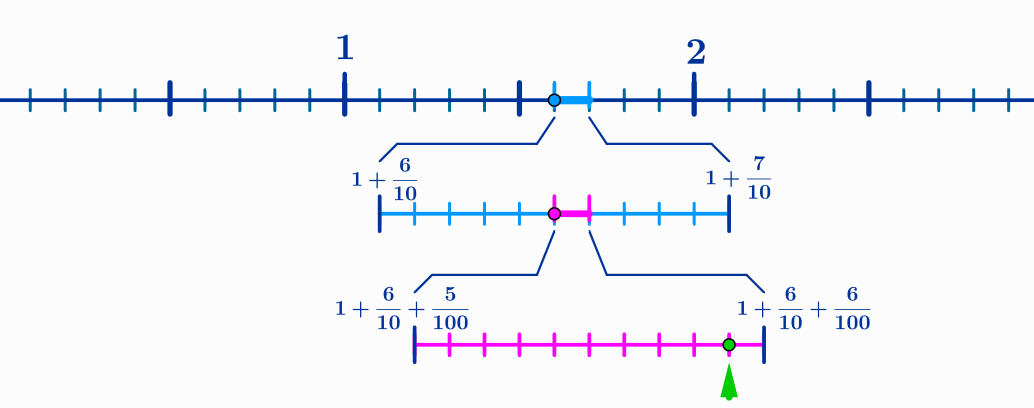
\includegraphics[width=\linewidth]{frac_decimales_demi-droite_zoom.PNG}
\end{center}
\end{Mt}

% \section{Les savoir-faire du parcours}

% \begin{CpsCol}
% \begin{itemize}
% \item Savoir écrire une fraction décimale.
% \item Savoir compléter une égalité de fractions décimales.
% \item Savoir comparer une fraction décimale à l'unité.
% \item Savoir décomposer une fraction décimale.
% \item Savoir encadrer une fraction décimale par deux entiers consécutifs.
% \item Savoir ajouter des fractions décimales.
% \item Savoir utiliser des fractions décimales.
% \item Savoir repérer une fraction décimale sur une demi-droite graduée.
% \item Savoir placer une fraction décimale sur une demi-droite graduée.
% \end{itemize}
% \end{CpsCol}

% \end{document}

\end{pageCours} 
\begin{pageAD} 
 

\Sf{Connaitre le vocabulaire des opérations}
 
  
\begin{ExoCad}{Communiquer.}{1234}{2}{0}{0}{0}{0}

 
\end{ExoCad}

\Sf{Connaitre les règles de priorités}

\begin{ExoCad}{Calculer.}{1234}{0}{0}{0}{0}{0}

 
 
\end{ExoCad}

\begin{ExoCad}{Calculer.}{1234}{0}{0}{0}{0}{0}

 
\end{ExoCad}


\Sf{Utiliser la distributivité}

\begin{ExoCad}{Représenter. Calculer.}{1234}{0}{0}{0}{0}{0}

 
 
\end{ExoCad}

\begin{ExoCad}{Calculer.}{1234}{0}{0}{0}{0}{0}

 
\end{ExoCad}

 
\end{pageAD}


%%%%%%%%%%%%%%%%%%%%%%%%%%%%%%%%%%%%%%%%%%%%%%%%%%%%%%%%%%%%%%%%%%%
%%%%  Niveau 1
%%%%%%%%%%%%%%%%%%%%%%%%%%%%%%%%%%%%%%%%%%%%%%%%%%%%%%%%%%%%%%%%%%%
\begin{pageParcoursu} 

 %%%%%%%%%%%%%%%%%%%%%%%%%%%
\begin{ExoCu}{Représenter.}{1234}{2}{0}{0}{0}{0}


\end{ExoCu}
%%%%%%%%%%%%%%%%%%%%%%%%%%%
\begin{ExoCu}{Représenter.}{1234}{2}{0}{0}{0}{0}


\end{ExoCu}
%%%%%%%%%%%%%%%%%%%%%%%%%%%
\begin{ExoCu}{Représenter.}{1234}{2}{0}{0}{0}{0}

\end{ExoCu}


%%%%%%%%%%%%%%%%%%%%%%%%%%%
\begin{ExoCu}{Raisonner.}{1234}{2}{0}{0}{0}{0}

\end{ExoCu}

%%%%%%%%%%%%%%%%%%%%%%%%%%%
\begin{ExoCu}{Représenter.}{1234}{2}{0}{0}{0}{0}


\end{ExoCu}


\end{pageParcoursu}

  
%%%%%%%%%%%%%%%%%%%%%%%%%%%%%%%%%%%%%%%%%%%%%%%%%%%%%%%%%%%%%%%%%%%
%%%%  Niveau 2
%%%%%%%%%%%%%%%%%%%%%%%%%%%%%%%%%%%%%%%%%%%%%%%%%%%%%%%%%%%%%%%%%%%



\begin{pageParcoursd} 
 
%%%%%%%%%%%%%%%%%%%%%%%%%%%%%%%%%%%%%%%%%%%%%%%%%%%%%%%%%%%%%%%%%%%
\begin{ExoCd}{Représenter.}{1234}{2}{0}{0}{0}{0}


 
\end{ExoCd}

 
%%%%%%%%%%%%%%%%%%%%%%%%%%%%%%%%%%%%%%%%%%%%%%%%%%%%%%%%%%%%%%%%%%%
\begin{ExoCd}{Chercher.communiquer.}{1234}{2}{0}{0}{0}{0}



\end{ExoCd}


%%%%%%%%%%%%%%%%%%%%%%%%%%%%%%%%%%%%%%%%%%%%%%%%%%%%%%%%%%%%%%%%%%%
\begin{ExoCd}{Représenter. Raisonner.}{1234}{2}{0}{0}{0}{0}


\end{ExoCd}

 %%%%%%%%%%%%%%%%%%%%%%%%%%%%%%%%%%%%%%%%%%%%%%%%%%%%%%%%%%%%%%%%%%%
\begin{ExoCd}{Représenter. Raisonner.}{1234}{2}{0}{0}{0}{0}


\end{ExoCd}
 
%%%%%%%%%%%%%%%%%%%%%%%%%%%%%%%%%%%%%%%%%%%%%%%%%%%%%%%%%%%%%%%%%%%
\begin{ExoCd}{Représenter. Raisonner.}{1234}{2}{0}{0}{0}{0}


\end{ExoCd}
 
\end{pageParcoursd}

%%%%%%%%%%%%%%%%%%%%%%%%%%%%%%%%%%%%%%%%%%%%%%%%%%%%%%%%%%%%%%%%%%%
%%%%  Niveau 3
%%%%%%%%%%%%%%%%%%%%%%%%%%%%%%%%%%%%%%%%%%%%%%%%%%%%%%%%%%%%%%%%%%%
\begin{pageParcourst}

%%%%%%%%%%%%%%%%%%%%%%%%%%%%%%%%%%%%%%%%%%%%%%%%%%%%%%%%%%%%%%%%%%%
\begin{ExoCt}{Représenter.}{1234}{2}{0}{0}{0}{0}

 

\end{ExoCt}

%%%%%%%%%%%%%%%%%%%%%%%%%%%%%%%%%%%%%%%%%%%%%%%%%%%%%%%%%%%%%%%%%%%
\begin{ExoCt}{Représenter. Raisonner.}{1234}{2}{0}{0}{0}{0}
 
 


\end{ExoCt}


%%%%%%%%%%%%%%%%%%%%%%%%%%%%%%%%%%%%%%%%%%%%%%%%%%%%%%%%%%%%%%%%%%%
\begin{ExoCt}{Raisonner.}{1234}{2}{0}{0}{0}{0}
 
\end{ExoCt}

%%%%%%%%%%%%%%%%%%%%%%%%%%%%%%%%%%%%%%%%%%%%%%%%%%%%%%%%%%%%%%%%%%%
\begin{ExoCt}{Représenter.}{1234}{2}{0}{0}{0}{0}

 

\end{ExoCt}

%%%%%%%%%%%%%%%%%%%%%%%%%%%%%%%%%%%%%%%%%%%%%%%%%%%%%%%%%%%%%%%%%%%
\begin{ExoCt}{Représenter.}{1234}{2}{0}{0}{0}{0}

 

\end{ExoCt} 
 
\end{pageParcourst}

%%%%%%%%%%%%%%%%%%%%%%%%%%%%%%%%%%%%%%%%%%%%%%%%%%%%%%%%%%%%%%%%%%%
%%%%  Brouillon
%%%%%%%%%%%%%%%%%%%%%%%%%%%%%%%%%%%%%%%%%%%%%%%%%%%%%%%%%%%%%%%%%%%


\begin{pageBrouillon} 
 
\ligne{32}



\end{pageBrouillon}

%%%%%%%%%%%%%%%%%%%%%%%%%%%%%%%%%%%%%%%%%%%%%%%%%%%%%%%%%%%%%%%%%%%
%%%%  Auto
%%%%%%%%%%%%%%%%%%%%%%%%%%%%%%%%%%%%%%%%%%%%%%%%%%%%%%%%%%%%%%%%%%%


%%%%%%%%%%%%%%%%%%%%%%%%%%%%%%%%%%%%%%%%%%%%%%%%%%%%%%%%%%%%%%%%%%%
\begin{pageAuto} 


\begin{ExoAuto}{Raisonner.}{1234}{2}{0}{0}{0}{0}

 
%%%%%%%%%%%%%%%%%%%%%%%%%%%%%%%%%%%%%%%%%%%%%%%%%%%%%%%%%%%%%%%%%%%
\end{ExoAuto}

\begin{ExoAuto}{Raisonner.}{1234}{2}{0}{0}{0}{0}
  

\end{ExoAuto}

%%%%%%%%%%%%%%%%%%%%%%%%%%%%%%%%%%%%%%%%%%%%%%%%%%%%%%%%%%%%%%%%%%%
\begin{ExoAuto}{Raisonner.}{1234}{2}{0}{0}{0}{0}

 
 

\end{ExoAuto}

 
%%%%%%%%%%%%%%%%%%%%%%%%%%%%%%%%%%%%%%%%%%%%%%%%%%%%%%%%%%%%%%%%%%%
\begin{ExoAuto}{Raisonner.}{1234}{2}{0}{0}{0}{0}

 
 

\end{ExoAuto}


\end{pageAuto}
